\documentclass{article}
\usepackage[utf8]{inputenc}

\title{Discrete Systems}
\author{Carli Peters and Lindsay Amendola}
\date{22 December 2020}
\usepackage{indentfirst}
\usepackage{graphicx}
\begin{document}

\maketitle

\section{Introduction}
The topic that we did our final project on is discrete systems, which is a system with a number of states that is countable and changes at a discrete set of points in time. Within discrete systems, changes occur in discrete steps. We can call these steps $k = 0,1,2,...i.$ The state of the system at time $i+1$ depends on the state of the system at all the previous times: \cite{shapiro2018scientific}
$$
n_{i+1}=f(n_0,n_1,n_2,...,n_i).
$$
These states can occur in multiple steps, as shown above, or can be done in a single step. The single step process is where the state of the system at $i+1$ only depends on the state of the previous step $i$:
$$
n_{i+1}=f(n_i)
$$
The single steps process of the system is also known as the fixed point iteration. It is also often used in the real world. \cite{shapiro2018scientific}
\subsection{Motivation}
A real life example on how discrete systems are used can be seen in the medical field. In the modern world, people rely on medications to improve their health or heal a wound. When medication is prescribed to be taken daily, a new dosage enters the body everyday. However, each time a new dosage is taken, there is still some medication left in the body that adds up in steps each time a dosage is taken. This process continues until there is enough of the dosage in the body that the medicine no longer has to be taken. The medical professionals who are giving the patients the doses can use fixed point iteration to see how much of the dose is left from the previous day for each day going forward. These iterations can then be plotted on a cobweb plot, which shows us what is happening at each iteration, or in this case, each day the patient is receiving medicine. 
\begin{figure}
    \centering
    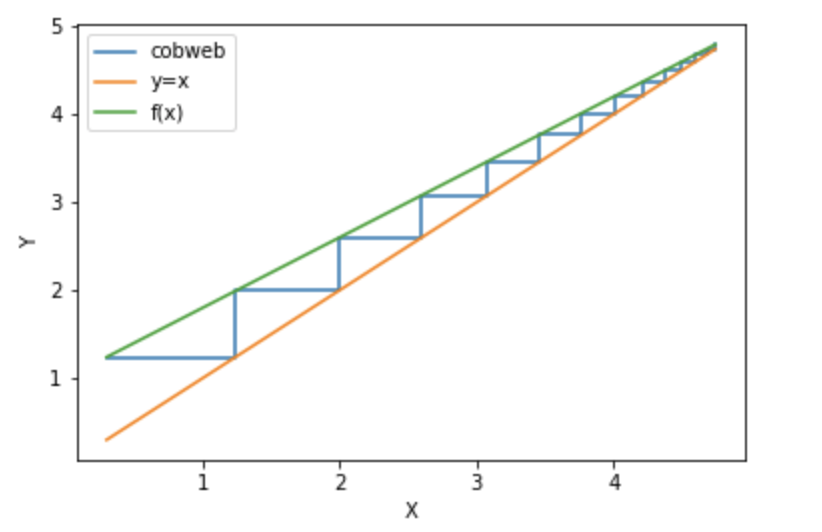
\includegraphics[width=8cm]{cobweb.png}
    \caption{This cobweb plot portrays how the fixed point iterations vary from day to day by taking discrete steps}
    \label{fig:Cobweb Plot for Medication Use}
\end{figure}

\subsection{Main Goals}
The main goals for the project are to see how each of the topics within discrete systems relate to one another. For instance, we can use how changes occur in discrete steps to look into other important points with discrete systems. Using the equation $n_{i+1}=f(n_0,n_1,n_2,...,n_i)$, we can see the iterations within cobweb plots, which can lead to convergence to a single fixed point. Discrete systems can also converge into patterns, which is seen in period 3 cycles that converge to three points and repeats every three iterations between those same three points. Furthermore, bifurcation diagrams can show the changes of fixed points in regard to a parameter in the function that also changes.

\subsection{Brief Summary}
Throughout the rest of the paper, we will be talking about the approaches we took to obtain the result of seeing how all the points in discrete systems relate to one another. We will go more in depth about cobweb plots, which show the reader what is happening at each iteration. This then leads into period 3 cycles, which is a system that converges to a sequence of three points rather than one fixed point. \cite{shapiro2018scientific} An image of this instance is shown in Figure 2:
\begin{figure}[htp]
    \centering
    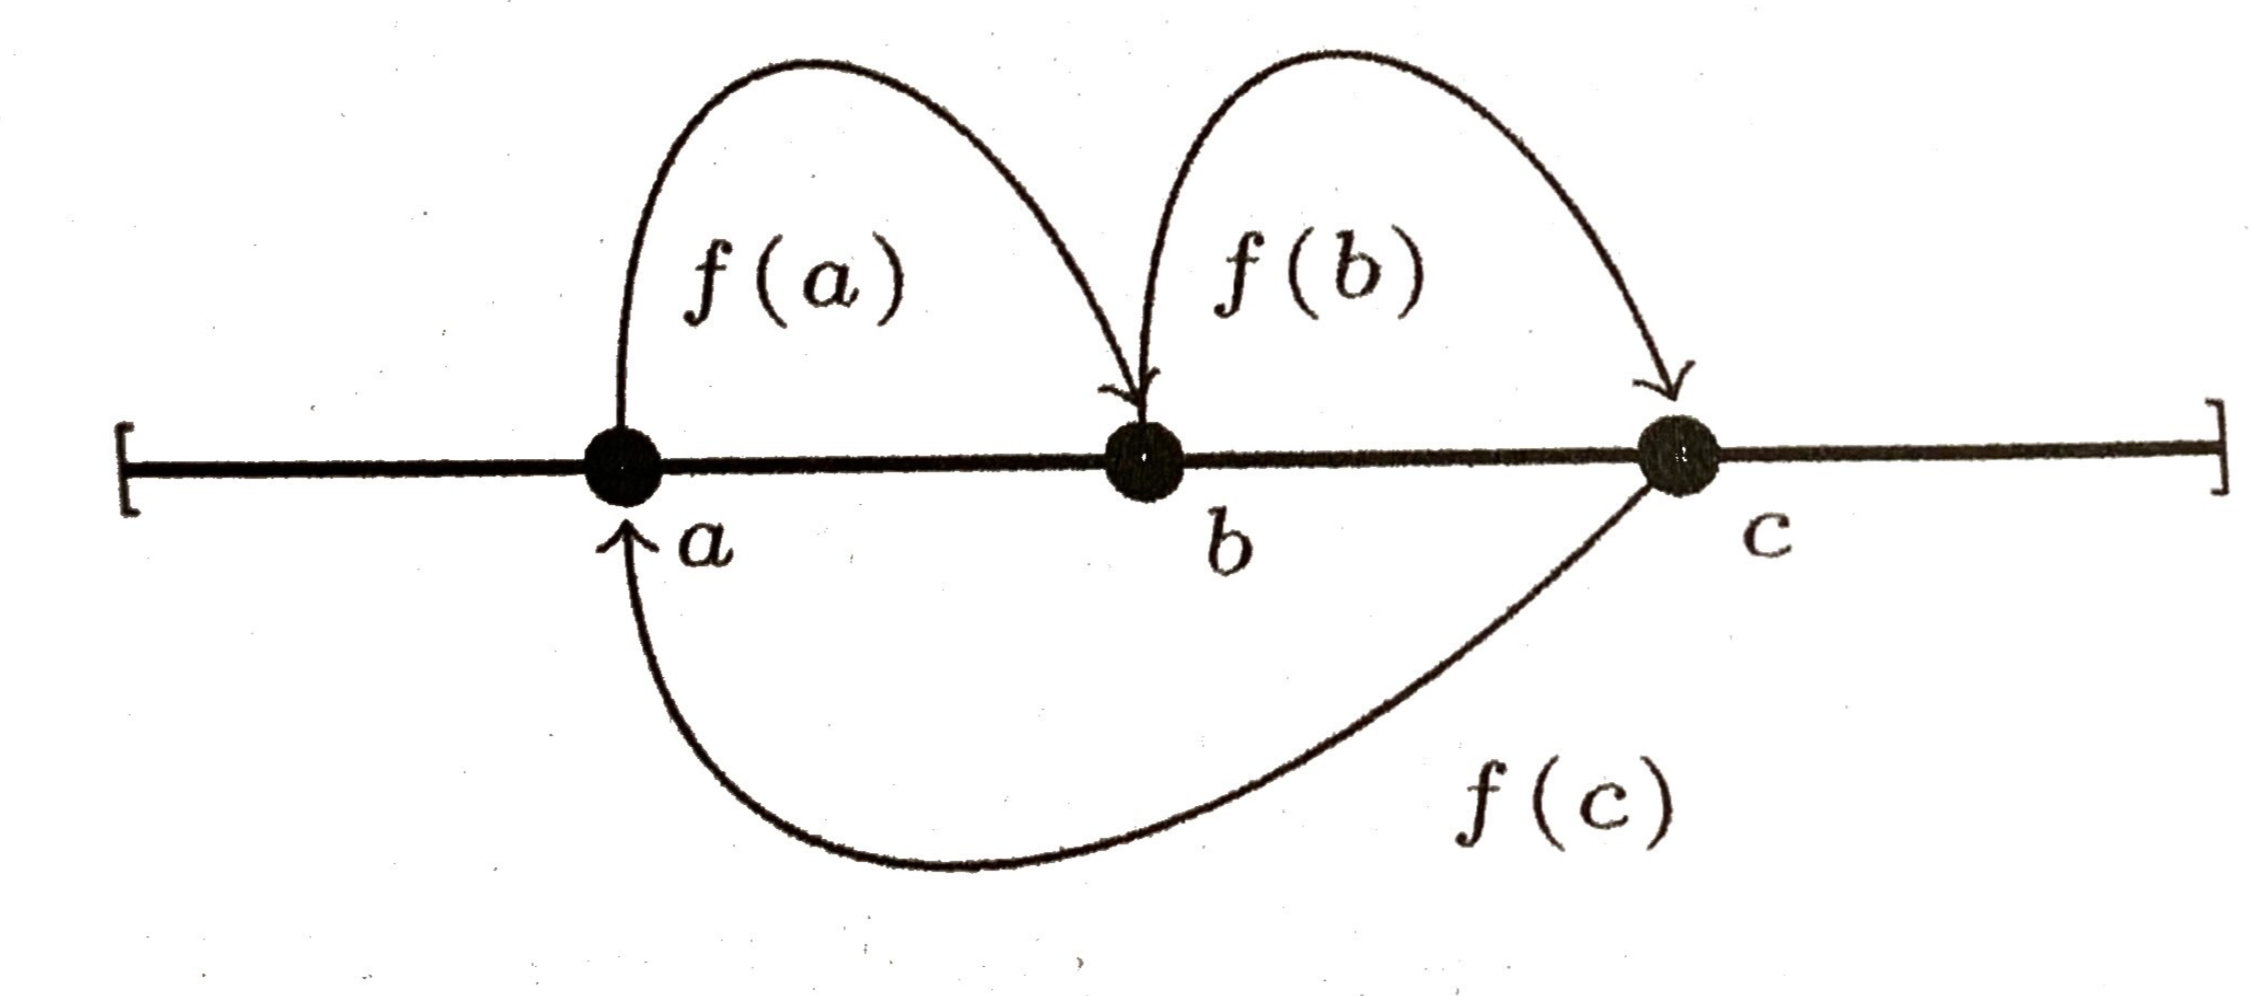
\includegraphics[width=8cm]{period3cycle.png}
    \caption{This portrays the system converging to a sequence of 3 points}
    \label{fig:Period 3 Cycle}
\end{figure}

Sometimes, discrete systems do not converge to one fixed point or go in a cycle of converging to the same three points. This is then indicating chaos, which is then looked into using a logistic map, which uses the equation:
$$
x_{n+1}=ax_n(1-x_n)
$$
Logistic maps can also help us see when bifurcation takes place, which is when two or more points tend to suddenly appear when $a$ is increased past 3. \cite{weisstein2001logistic} An image of a bifurcation diagram is shown in figure 3:
\begin{figure}[htp]
    \centering
    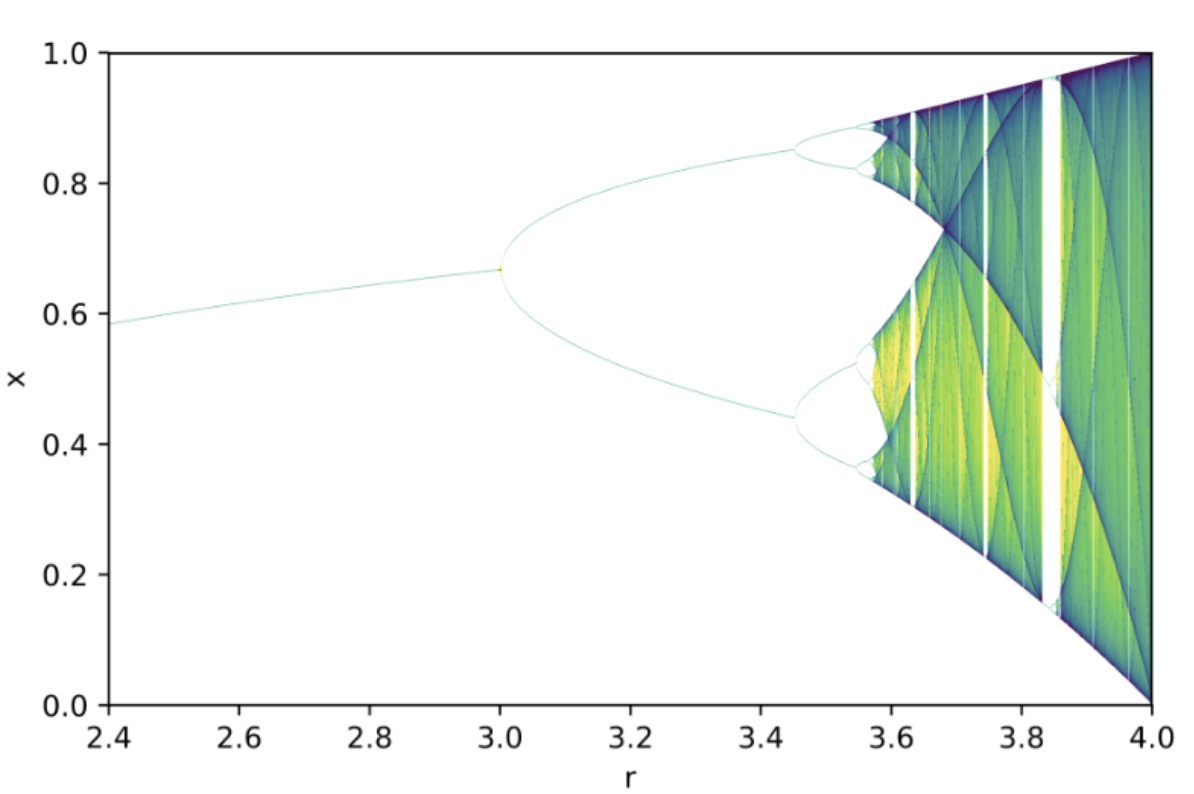
\includegraphics[width=8cm]{bifurcation.png}
    \caption{Bifurcation Diagram}
    \label{fig:Bifurcation Diagram}
\end{figure}

Besides the main topics of discrete systems, we will also go on to talk about the approach we took to solve problems related to each topic. Within these results, it will be shown how each exercise also related to one another and all tied together in the end. 

\section{Approach}
While reading about discrete systems in chapter 40 of Bruce Shapiro's textbook \emph{Scientific Computation: Python 3 Hacking for Math Junkies}, we recognized how all the main topics in the chapter related to one another. Besides just knowing that the topics tied together, it is important to also be able to show how each topic in the chapter comes together by going through the concepts of the textbook and doing the exercises on our own.

\subsection{Tent Map}
The first concept portrayed was plotting a tent map to help determine the locations of the fixed points in the given function. Tent maps are typically defined on a given interval and then a piecewise function is provided to show the functions that are being used to create the tent map. Furthermore, when the tent map is plotted with the cobweb plot, we are able to see the iterations that lead to the point of convergence between the function and the diagonal line $y=x$. The function can converge to a single fixed point or a pattern between points. An example of a tent map is shown in Figure 4:
\begin{figure}[htp]
    \centering
    \includegraphics[width=8cm]{tentmap.png}
    \caption{This shows what a tent map should look like}
    \label{fig:Tent Map}
\end{figure}

\subsection{Bifurcation Diagram}
After providing the locations of the fixed points of a tent map, we were asked to provide a bifurcation diagram of the logistic map. A logistic map is similar to a tent map, in which it helps show where fixed points should occur. Bifurcation diagrams then work as a great visualization to show a logistic map's chaotic regime. \cite{weisstein2001logistic} You can run a logistic map $N$ amount of times to generate a large amount of ending values. A bifurcation diagram shows the behavior and amount of points within the pattern in regards to the changing parameter of the function. The parameter is the fixed constant given to the function. As the parameter changes, the amount of points can increase as well as their values changing. \cite{shapiro2018scientific}

\subsection{Cobweb Plots}
A cobweb plot requires a python function the converges with the line $y=x$. As this point of convergence is a fixed point, the cobweb plot will show the behavior of the iterations as the function reaches that fixed point. Within the function, one would need $f$, which is the name of the function that has to be plotted. Along with $f$, a value for $x0$ is needed. The $x0$ is the initial value of $x$ from the function. From here, we have to see how many iterations have to be performed, which is where the value $n$ comes in. For both the $x$ axis and the $y$ axis, the minimum and maximum values are needed. With all of these initial values a cobweb plot with any specific function can be called. \cite{shapiro2018scientific}

\section{Results}
While doing specific examples in the textbook, we noticed how these exercises were linked to one another. A recurring theme was that one question would ask about one topic, the next question would ask about a different topic, and then the following question would bring the previous two questions together. Specific instances of these occurrences will be shown throughout this section of the paper. 

\subsection{Tent Maps with Bifurcation}
The initial problem we had to solve was first seeing a tent map being defined on an interval with a given piecewise function. In the given piecewise function, a value $a$ is being multiplied by different values, depending on if $x$ is bigger or smaller than $\frac{1}{2}$. $a$ is a real, positive constant, that is $>0$. The value of $a$ will then determine whether the function has one, or multiple fixed points. In this instance, if $a>1$, there would be two fixed points and the goal was to find the location of the two fixed points. To find the location, one must define the tent map and then make lists for the inputs and outputs. We must add on to the list by making a for loop and appending the input and output values. However, for the inputs, the values being added to the list may differ, depending on whether $y$, which is provided in the tent map definition is bigger or smaller than a certain value. The inputs and outputs would then be printed as a list of fixed point locations. 
\begin{figure}[htp]
    \centering
    \includegraphics[width=8cm]{function.png}
    \caption{Specific Function of a Tent Map}
    \label{fig:Tent Map Function}
\end{figure}
\begin{figure}[htp]
    \centering
    \includegraphics[width=8cm]{list.png}
    \caption{List of Fixed Points}
    \label{fig:Tent Map Fixed Point List}
\end{figure}

First, we were able to determine the locations of two fixed points. The next step here is to generate a bifurcation diagram. A bifurcation diagram is meant to show the visited values or the approached values. These values can consist of fixed points, periodic orbits, or chaos. These values appear in the discrete system as a function of a bifurcation parameter within the system. Again, this parameter is a fixed constant given to the function. The bifurcation diagram overall shows the visualization of all the fixed points and periodic orbits. \cite{boeing2018pynamical} In order to create a bifurcation diagram, we must form a parameter with a linspace consisting of a starting point and ending point for $x$ along with another number to determine the pixel quality of the bifurcation diagram. We then define $m$ to be $1$ and then define $X$ and $Y$ as empty lists that have to be appended as we go through the for loops. When it is time to plot, the accumulated lists of $X$ and $Y$ will be plotted. An image of what the bifurcation diagram should look like it provided in Figure 7:
\begin{figure}[htp]
    \centering
    \includegraphics[width=8cm]{diagram.png}
    \caption{Bifurcation Diagram}
    \label{fig:Bifurcation Diagram}
\end{figure}

These two concepts listed above can then come together by making a bifurcation diagram with the tent map previously mentioned. The process forming this bifurcation diagram is very similar to how it was formed in the previous paragraph. The only difference would be the starting point in the linspace and the pixel quality. Once the $y$ value is at $\frac{1}{2}$ like in the original tent map function, more fixed points occur.
\begin{figure}[htp]
    \centering
    \includegraphics[width=8cm]{tentbi.png}
    \caption{Bifurcation Diagram of Tent Map}
    \label{fig:Bifurcation Diagram of Tent Map}
\end{figure}

\subsection{Tent Maps with Cobweb Plots}
Before plotting a cobweb plot for the tent map, we first defined a function for the cobweb plot to see the iterations of the cosine function. After plotting the $cos(x)$ function and the line $y=x$ we could see that the line and the curve of cosine converged at a point between $x=0.7$ and $x=0.8$. We can confirm that this point is a fixed point by plotting the cobweb and seeing the behavior of each iteration.
\begin{figure}[htp]
    \centering
    \includegraphics[width=8cm]{cobweb2.png}
    \caption{This is the cobweb plot for $cos(x)$ on the interval [0,1.5]}
    \label{fig:Cobweb}
\end{figure}

For the cobweb plot, $x_0$ was given the value of $1$. As shown in the figure above, the next iteration is between the $x$ values of $0.5$ and $0.6$. This was found by starting at the initial value of $x$ on the graph of $cos(x)$ and moving horizontally to the line of $y=x$ and then back vertically to the graph of $cos(x)$. By repeating this process of moving horizontally to the diagonal line and then vertically to the graph of cosine, the next iteration can be found. Eventually the iterations continue in a spiral pattern that seems to converge at the same point where the graph of cosine and the diagonal line intersect. 

The next exercise required us to use the concepts and code used for plotting a cobweb for the cosine function but to do this for the tent map defined in the first exercise. To incorporate the tent map into our code we needed to define the piecewise function using an if-else statement for the values of x that were given for each individual line. There was also a parameter $a$ that each line was being multiplied by. We choose the parameter $a=2$. The first part of the piecewise function was $a(x)$ for $x<\frac{1}{2}$. The other line $a(1-x)$ for $x>=\frac{1}{2}$ intersects with the diagonal line, which is where the fixed point should be. Based on the bifurcation diagram of the tent map we generated, we know what to expect for the value of the fixed point and the amount of points in the pattern of convergence depending on the value of the parameter. With a parameter $a<3$ there is only one fixed point and if the parameter $a<1$, that fixed point would be at $x=0$. The cobweb plot below shows the iterations of the cobweb plot of the tent map with initial value $x_0= 0.1$ and parameter $a=2$. 


\begin{figure}[htp]
    \centering
    \includegraphics[width=8cm]{cobweb3.png}
    \caption{This is the cobweb plot for the tent map on the interval [0,1]}
    \label{fig:Cobweb plot}
\end{figure}

The cobweb plot that was generated showed a spiral pattern for the iterations as the iterations followed the process described previously in this paper. As it is difficult to see the exact point that the iterations converge to, the iterations are nearing the point of convergence of the piecewise function and the line $y=x$. While increasing the value for $n$, which is the amount of fixed point iterations we want performed, the cobweb plot does not show a noticeable difference from the figure above.  

 

\section{Discussion and Conclusions}
From doing specific examples about the main topics of discrete systems, we were able to see how the topics in the exercises related to one another. The topics did not blend together as seamlessly as initially predicted, but they still relate to one another.

\subsection{Discuss Main Results}
The main results of our project showed how tent maps, bifurcation diagrams, and cobweb plots all relate to one another and how more than one of these can be used together. Out of these three topics, the tent map was the function that linked everything else together. The bifurcation diagram showed the behavior of the fixed point as the fixed constant in the function changes. The cobweb plot shows the behavior at each iteration as the function nears the fixed point or points of convergence. 


Bifurcation diagrams are able to show the behavior of a fixed point as the parameter changes and this can help confirm where the fixed point should be on the cobweb diagram. While working through the exercises we were able to use the bifurcation diagram of the tent map to help confirm that our cobweb plot of the tent map was correct or incorrect. While generating a cobweb plot for the tent map it became evident that the initial value for $x$ and the random value for the fixed constant parameter $a$ has a large impact on how the cobweb plot looks. Using the bifurcation diagram we were able to see that if the parameter was $2$ there would be one fixed point at about $x=0.5$. For the value of the parameter $a$ on the interval$[0,1]$ there would be one fixed point at $x=0$. At first with the cobweb plot, the fixed point at $x=0$ seemed incorrect. However, by using the bifurcation diagram we were able to see that this in fact was accurate. The value of the parameter and the initial value can alter the cobweb plot.

It is also important to remember that the intervals given in the instructions for the exercises go along with specific functions, not the overall plot. A few instances occurred where initial values were picked that did not fall within the correct interval given. This was an issue that had to be addressed multiple times within our work.

\subsection{Future Considerations}
Possible approaches that someone else, or future us, might attempt would be to figure out how to use a function of a period 3 cycle or larger and see how its cobweb plot would correlate with a bifurcation diagram. By doing this, we could see how different types of functions would produce different cobweb plots and bifurcation diagrams. We could also go more in depth with the use of initial values for $x$ or for the parameter $a$ and how these values affect the diagrams being produced. 


\pagebreak{1}
\cite{weisstein2001logistic}
\cite{shapiro2018scientific}
\cite{boeing2018pynamical}
\bibliographystyle{unsrt}
\bibliography{name.bib}

\end{document}
